Magnitude analysis is well-suited for analyzing low-level behavior, yet most research questions are at a higher level. The research question ``How often are refactorings performed?'' cannot be answered via magnitude analysis alone, as refactorings can be triggered through tens of different commands. These commands first need to be categorized, after which magnitude analysis can be used. When focusing on a concrete sub-task, such as refactoring, it may be easy to categorize activities. In this case, all refactoring commands, such as pull-up or extract method, can be classified as refactorings. However, when focusing on more general behavior, such as editing, navigating, and searching, categorizations can be difficult. It is impossible to say, for instance, from a single click in the file explorer whether that click represents a search, as the developers browses a few promising files, or a navigation, as he implicitly opens a type declaration of a variable he was just browsing. Thus, categorization at the individual action level is necessarily noisey data, which effects the strength of conclusions that can be made from it.

\begin{figure*}[t]
 \centering
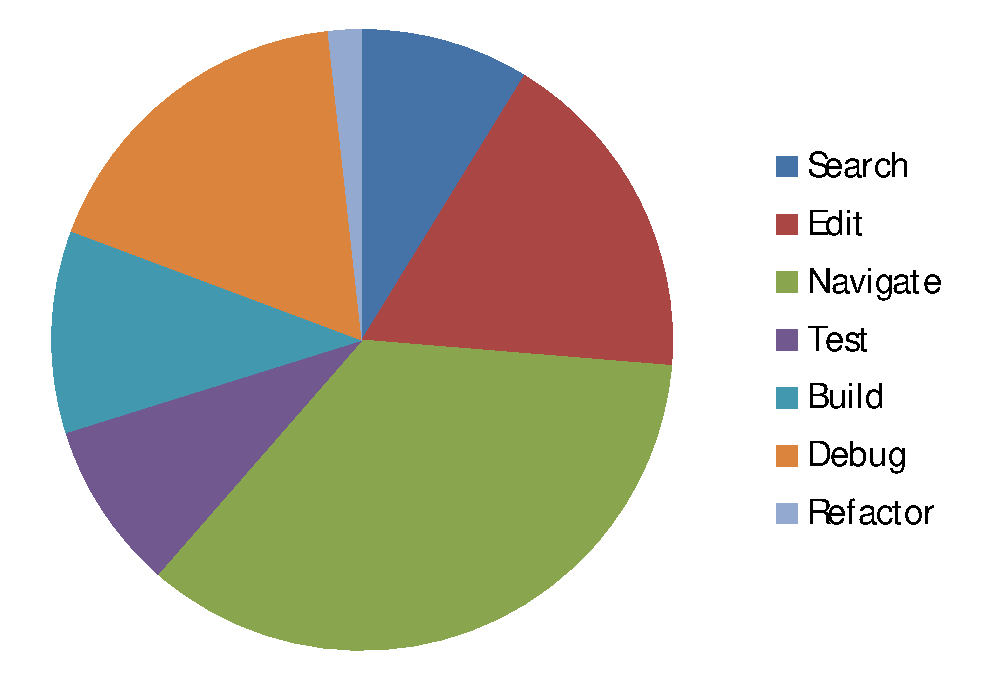
\includegraphics[width=0.5\columnwidth]{../Graphics/activityCategorization.pdf}
%\caption{Pairwise matches across categories, including matching and mismatching pairs.}
\label{fig:category}
\end{figure*}